\documentclass[a4paper,14pt]{report}
\usepackage[utf8]{inputenc}
\usepackage[italian]{babel}

\usepackage{amsmath}
\usepackage{graphicx}
\usepackage{indentfirst}

\title{Ma sarà vero che $1+1=2$?\\[3em]
\small Tesina AA 2020/2021}
\author{Paolo Caressa}
\date{Maggio 2021}

\begin{document}

\maketitle

\begin{abstract}
In questa tesina ci proponiamo di approfondire e rispondere a un enigma fondamentale della conoscenza umana. Per il sollievo di tutti, la risposta sarà positiva, ma si rimanda alle conclusioni per una sua più estesa articolazione.
\end{abstract}

\tableofcontents

\pagestyle{headings}

\chapter*{Introduzione}

Si fa presto a dire $1+1=2$ ma è realmente vero? e, se sì, perché? A queste gravi ed annose domande si propone di rispondere questa breve ma, speriamo, incisiva tesina.

Collegamenti interdisciplinari:
\begin{itemize}
    \item Filosofia: l'Uno di Plotino.
    \item Geografia: l'una di notte che ore sono in Guatemala?
    \item Italiano: {\em Uno, nessuno e centomila} di Pirandello.
    \item Scienze: la Luna.
    \item Storia: ma dopo l'1 a.C.\ è venuto l'anno 0 o l'anno 1?
\end{itemize}

\chapter{Il problema}

\section{Gli assiomi di Peano}

Come classicamente noto (cfr.\ \cite{peano}), i numeri naturali si caratterizzano formalmente come gli elementi di un insieme tale che
\begin{enumerate}
    \item Esista almeno un elemento $0\in{\mathbf N}$.
    \item Sia data una funzione $s\colon{\mathbf N}\to{\mathbf N}$.
    \item La funzione $s$ sia iniettiva: se $s(n)=s(m)$ allora $n=m$.
    \item $0$ non sia nell'immagine di $s$, cioè non esista alcun $n\in{\mathbf N}$ tale che $s(n)=0$.
    \item Se $M\subset{\mathbf N}$ e se:
    \begin{itemize}
        \item $0\in M$
        \item Per un qualsiasi $n\in M$ si ha necessariamente che anche $s(n)\in M$
    \end{itemize}
    allora $M={\mathbf N}$.
\end{enumerate}
Queste cinque proprietà si chiamano {\em assiomi di Peano}.

I numeri naturali che normalmente sono denotati da numerali, cioè da stringhe finite di cifre decimali interpretate nella notazione posizionale e in base 10, vanno fatti corrispondere a termini della teoria di Peano, che denotano elementi del dominio $\mathbf N$ del quale essa parla, nel modo seguente:
\begin{align*}
    0 &\to 0, \\
    1 &\to s(0), \\
    2 &\to s(1)=s(s(0)), \\
    3 &\to s(2)=s(s(1))=s(s(s(0))), \\
    \cdots & \cdots \cdots \cdots
\end{align*}
Nel presente studio assumeremo implicitamente questa corrispondenza, che peraltro ci è necessaria solo nelle sue tre prime istanze.

\section{La somma}

Definiamo la somma di due numeri ricorsivamente come
\[
\label{eq-dedekind}
\begin{cases}
    n+0 = n, \\
    n+s(m) = s(n+m)
\end{cases}
\]
Come noto (cfr.\ \cite{dedekind}) questa operazione è univoca e ben definita: la dimostrazione di questo fatto richiede tutti e cinque i precedenti assiomi di Peano.

\section{Formulazione del problema}

L'equazione $1+1=2$ si traduce nella seguente, usando l'assiomatica peanea:
\[
    s(0)+s(0) = s(s(0))
\]

Infatti il numero $1$ è corrisponde al successore dello zero, dunque al termine $s(0)$ della teoria di Peano. Il numero $2$ corrisponde invece al successore di $1$, dunque al termine $s(1)=s(s(0))$ della teoria di Peano.

\chapter{Soluzione del problema}

Partiamo dall'espressione
\[
    s(0)+s(0)
\]
Applicando la definizione ricorsiva di Dedekind (\ref{eq-dedekind}) la riduciamo alla
\[
    s(s(0)+0)
\]
L'argomento della funzione $s$ più esterna è, sempre per la definizione ricorsiva di somma, pari a $s(0)$, col che abbiamo ridotto l'espressione a
\[
    s(s(0))
\]
che è proprio quel che volevamo dimostrare.

\chapter*{Conclusioni}

Stante l'assiomatica di Peano la questione è chiarita. Tuttavia sorge spontanea la domanda se esistano sistemi numerici più deboli di quello di Peano per i quali l'equazione non sia violata.

\`E questo il caso dell'anello delle classi di resti modulo 2 (cfr.\ \cite{gauss}), anche noto come ${\mathbf Z}_2$: in quel caso è noto che $1+1=0$, ma si tratta di una questione che va al di là dei limiti di tempo, spazio e complessità previsti per la presente nota.

\appendix
\chapter{Ritratti}

\begin{figure}[h!]
\centering
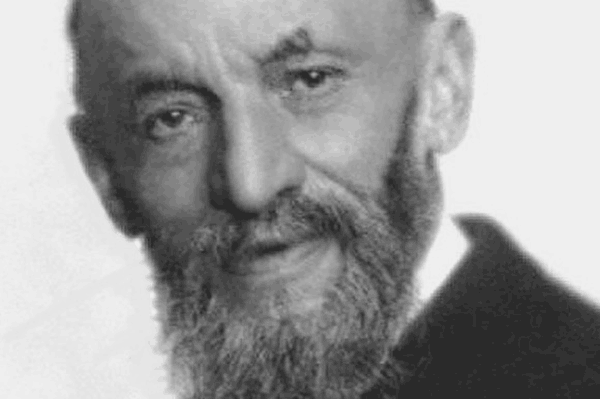
\includegraphics[width=.7\textwidth]{peano.png}
\caption{Giuseppe Peano}
\end{figure}

\begin{figure}[h!]
\centering
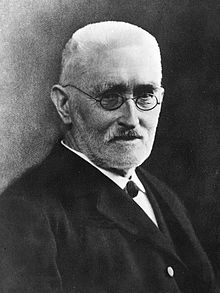
\includegraphics[width=.7\textwidth]{Richard_Dedekind_1900s.jpg}
\caption{Richard Dedekind}
\end{figure}

\begin{figure}[h!]
\centering
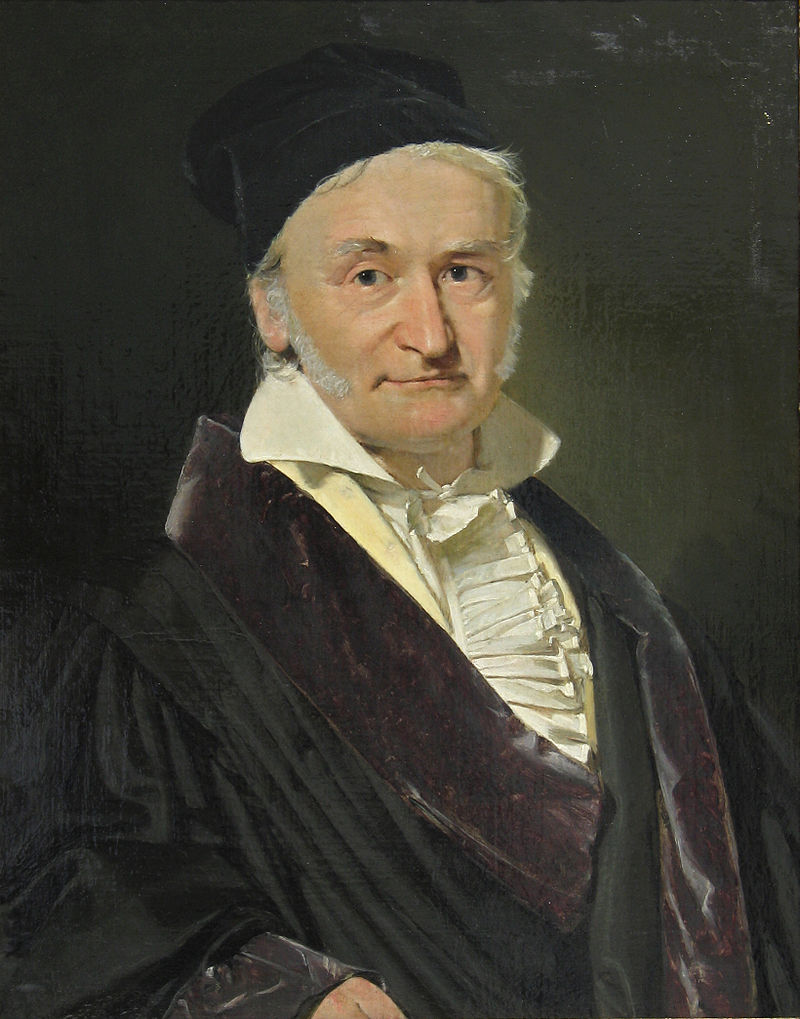
\includegraphics[width=.7\textwidth]{800px-Carl_Friedrich_Gauss_1840_by_Jensen.jpg}
\caption{Carl Friedrich Gauss}
\end{figure}

\begin{thebibliography}{99}

\bibitem%[Dedekind, 1888]
{dedekind} Richard Dedekind, {\it Was sind und was sollen die Zahlen?}, Braunschweig, 1888.

\bibitem%[Gauss, 1801]
{gauss} Carl Friedrich Gauss, {\it Disquisitiones Arithmeticae}, G\"ottingen, 1801.

\bibitem%[Peano, 1899]
{peano} Giuseppe Peano, {\em  Arithmetices principia, nova methodo exposita}, Torino, 1899.

\end{thebibliography}

\end{document}
